\section{Theorie}
\label{sec:Theorie}
Ultraschall bezeichnet longitudinale Schallwellen im Frequenzbereich von ca.
20\,kHz bis 1\,GHz, der oberhalb der Hörschwelle des Menschen liegt.
Die Erzeugung von Ultraschall kann zum Beispiel durch Anwendung des reziproken piezo-elektrischen
Effektes geschehen. In elektrischen Wechselfeldern können piezoelektrische Kirstalle, wie zum Beispiel Quarze,
zu Schwingungen, bei denen Ultraschall abgestrahlt wird, angeregt werden. Auch das Empfangen
von Ultraschall ist mit piezoelektrischen Kristallen möglich, da diese zu Schwingungen
angeregt werden, wenn jener auf den Kristall trifft.
Für weitere grundlegende Informationen zu Ultraschall kann \cite{VersuchsanleitungUS2}
herangezogen werden.\\
Es ist möglich, mithilfe von Ultraschall Geschwindigkeiten von Strömungen experimentell
zu bestimmen. Dabei spielt der Doppler-Effekt eine Rolle, da der Ultraschall auf
ein sich bewegendes Objekt trifft. Die Frequenz vergrößert sich, falls sich die Quelle auf den
Empfänger zubewegt oder falls sich der Empfänger der Quelle nähert. Entfernt sich die Quelle
hingegeben vom Beobachter oder andersherum so wird die Frequenz geringer. Dies lässt sich wie folgt
zusammenfassen:
\begin{equation}
  \nu_\text{B} = \nu_\text{S} \left(\frac{c \pm v_\text{B}}{c \mp v_\text{S}}\right)\,.
  \label{eqn:geschwindigkeit}
\end{equation}
Für Annäherung von Sender und Empfänger ist das obere Vorzeichen zu wählen, für
das Entfernen voneinander gilt das Untere. Die Frequenz, die der Beobachter msisst,
wird mit $\nu_\text{B}$ bezeichnet. Der Sender misst die Frequenz $\nu_\text{S}$, $c$ bezeichne
die Schallgeschwindigkeit des Mediums, in dem sich beide befinden. Die Geschwindigkeiten
relativ zum Medium seien mit $v_\text{B}$ für den Beobachter und $v_\text{S}$ für den
Sender bezeichnet. Diese Formel gilt nur, falls sich Beobachter und Empfänger geradlinig
aufeinander zu bewegen.\\
Diese Lage ist im Allgemeinen jedoch nicht gegeben. Wird zum Beispiel Ultraschall
genutzt, um eine Strömung zu untersuchen, so ergibt sich für die Frequenzverschiebung
\begin{equation}
  \Delta \nu = \nu_0 \frac{v}{c} \cos \alpha\,.
\end{equation}
Dies ist am Beispiel der Untersuchung von Blutkörpern in Abbildung \ref{fig:theorieskizze}
skizziert. Dabei ist $\alpha$ der Dopplerwinkel. Dieser berechnet sich durch
\begin{equation}
  \alpha=90°-\arcsin\left(\sin(\theta)\frac{c_{\symup{L}}}{c_{\symup{P}}}\right) \,,
  \label{eqn:dopplerwinkel}
\end{equation}
wobei $c_{\symup{L}}$ die Schallgeschwindigkeit in der Dopplerflüssigkeit und
$c_{\symup{P}}$ die Schallgeschwindigkeit im Dopplerprisma ist.

\begin{figure}
  \centering
  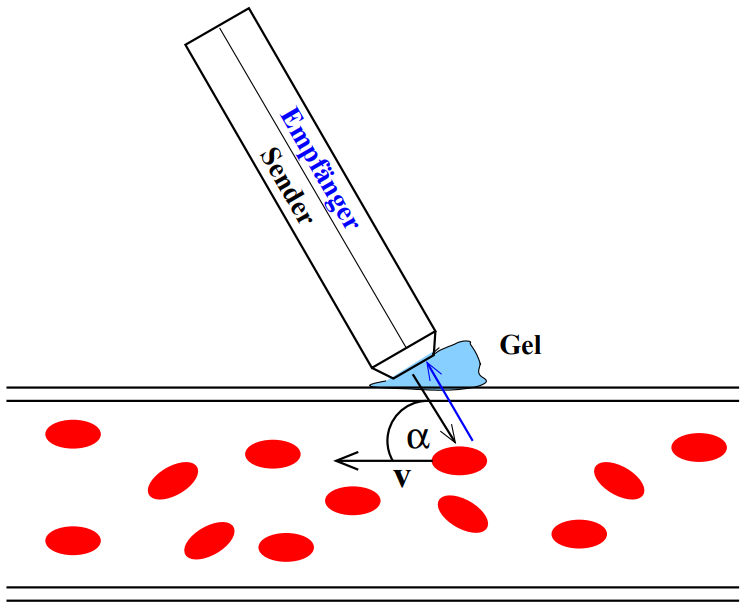
\includegraphics[width=200pt]{data/dopplerskizze.png}
  \caption{Schematische Darstellung der Untersuchung von Blutkörpern mit Ultraschall\,\cite{Versuchsanleitung}}
  \label{fig:theorieskizze}
\end{figure}
